% tikz_closure.tex -- the two schematics of Section 2.8, drawn in TikZ.
%   (a) Lemma 2.15: four centres pairwise at least 2 apart need a ball of radius
%       at least sqrt(3/2); the regular tetrahedron of edge 2 attains it.  If a
%       point x with |x| < sqrt(3/2) were closer to three centres y_1, y_2, y_3
%       than to the centre 0, the four points would lie in the ball of radius
%       |x| about x.  To scale (orthographic view).
%   (b) Lemma 2.12, in a plane section: a centre z can come close to c only in
%       a hole of the contact directions, and then |z| >= 4 cos(rho), rho the
%       angular radius of the hole (here rho = 50 degrees, so |z| >= 2.571).
%       The dashed circles of radius 2 about the contacts are the regions no
%       other centre may enter.  To scale.
% Build:  pdflatex tikz_closure.tex && pdftoppm -r 500 -png -singlefile tikz_closure.pdf ../figures/fig_tikz_closure
\documentclass[border=4pt]{standalone}
\usepackage{tikz,tikz-3dplot}
\usetikzlibrary{calc,arrows.meta,decorations.pathreplacing}
\usepackage[T1]{fontenc}
\usepackage{lmodern}
\definecolor{cblue}{HTML}{2A78D6}
\definecolor{corange}{HTML}{EB6834}
\definecolor{caqua}{HTML}{1BAF7A}
\definecolor{cink}{HTML}{0B0B0B}
\definecolor{cink2}{HTML}{52514E}
\definecolor{cink3}{HTML}{8B8A85}
\definecolor{cpanel}{HTML}{F4F3EF}
\begin{document}
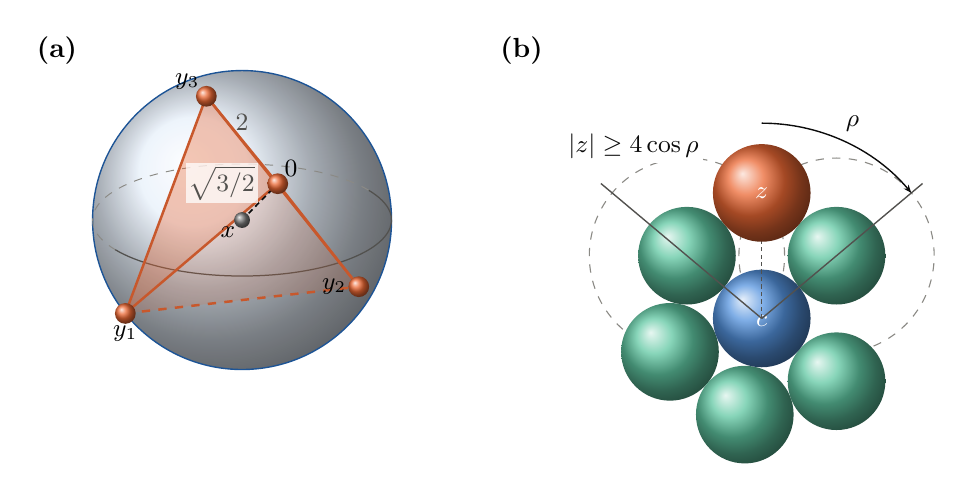
\begin{tikzpicture}[font=\small]
%% ------------------------------------------------------------------ (a)
\tdplotsetmaincoords{68}{118}
\begin{scope}[tdplot_main_coords, scale=1.55]
  \pgfmathsetmacro{\R}{sqrt(1.5)}
  \pgfmathsetmacro{\h}{1/sqrt(2)}
  % the ball of radius sqrt(3/2), shaded; an orthographic sphere is a disc
  \begin{scope}[tdplot_screen_coords]
    \shade[ball color=cblue!12, opacity=0.95] (0,0) circle (\R);
    \draw[cblue!70!black, line width=0.5pt] (0,0) circle (\R);
  \end{scope}
  % equator, back half dashed
  \tdplotdrawarc[tdplot_main_coords, dashed, cink3, line width=0.35pt]{(0,0,0)}{\R}{150}{330}{}{}
  \tdplotdrawarc[tdplot_main_coords, cink2, line width=0.45pt]{(0,0,0)}{\R}{-30}{150}{}{}
  % the regular tetrahedron of edge 2
  \coordinate (P0) at ( \h, \h, \h);
  \coordinate (P1) at ( \h,-\h,-\h);
  \coordinate (P2) at (-\h, \h,-\h);
  \coordinate (P3) at (-\h,-\h, \h);
  \coordinate (X)  at (0,0,0);
  \fill[corange, opacity=0.16] (P1) -- (P2) -- (P3) -- cycle;
  \fill[corange, opacity=0.24] (P0) -- (P1) -- (P3) -- cycle;
  \fill[corange, opacity=0.30] (P0) -- (P2) -- (P3) -- cycle;
  \draw[corange!85!black, line width=0.9pt, dashed] (P1) -- (P2);
  \foreach \a/\b in {P0/P1,P0/P2,P0/P3,P1/P3,P2/P3}
    \draw[corange!85!black, line width=0.9pt] (\a) -- (\b);
  % the radius from x to 0
  \draw[cink, line width=0.6pt, dash pattern=on 2pt off 1.4pt] (X) -- (P0);
  \begin{scope}[tdplot_screen_coords]
    \foreach \p in {P0,P1,P2,P3}
      \shade[ball color=corange] (\p) circle (0.085);
    \shade[ball color=cink!55] (X) circle (0.065);
  \end{scope}
  \node[above right=-1pt] at (P0) {$0$};
  \node[below=1pt] at (P1) {$y_1$};
  \node[left=1pt] at (P2) {$y_2$};
  \node[above left=-1pt] at (P3) {$y_3$};
  \node[below left=-1pt] at (X) {$x$};
  \path (P0) -- (P3) node[midway, above=0pt, cink2] {$2$};
  \path (X) -- (P0) node[pos=0.45, above left=0pt, fill=white, fill opacity=0.75,
    text opacity=1, inner sep=1pt, text=cink2] {$\sqrt{3/2}$};
\end{scope}
\node[font=\bfseries] at (-2.35,2.15) {(a)};
%% ------------------------------------------------------------------ (b)
\begin{scope}[xshift=6.6cm, yshift=-1.25cm, scale=0.62]
  \pgfmathsetmacro{\zr}{4*cos(50)}
  % exclusion circles of radius 2 about the contacts next to the hole
  \foreach \t in {40,140}
    \draw[cink3, dashed, line width=0.4pt] (\t:2) circle (2);
  % contact balls (radius 1) at distance 2
  \foreach \t in {40,140,200,260,320} {
    \shade[ball color=caqua!70] (\t:2) circle (1);
  }
  % the central ball
  \shade[ball color=cblue!80] (0,0) circle (1);
  \node[white] at (0,-0.05) {$c$};
  % the hole: rays at 40 and 140 degrees, and its angular radius
  \draw[cink2, line width=0.5pt] (0,0) -- (40:4.3);
  \draw[cink2, line width=0.5pt] (0,0) -- (140:4.3);
  \draw[cink2, line width=0.5pt, dash pattern=on 1.5pt off 1.2pt] (0,0) -- (90:\zr);
  \draw[cink, line width=0.5pt, -{Stealth[length=3pt]}] (90:4.0) arc (90:40:4.0);
  \node[cink] at (65:4.4) {$\rho$};
  % the centre in the hole, touching the two exclusion circles
  \shade[ball color=corange] (90:\zr) circle (1);
  \node[white] at (90:\zr) {$z$};
  \node[anchor=east, fill=white, inner sep=1.5pt, text=cink] at ($(90:\zr)+(-1.2,0.95)$)
    {$|z|\ge4\cos\rho$};
\end{scope}
\node[font=\bfseries] at (3.55,2.15) {(b)};
\end{tikzpicture}
\end{document}
